\documentclass[xcolor=dvipsnames]{beamer}

\usetheme{Darmstadt}
\usefonttheme[onlylarge]{structurebold}
\setbeamerfont*{frametitle}{size=\normalsize,series=\bfseries}
\setbeamertemplate{navigation symbols}{}

\usepackage[english]{babel}
\usepackage[cp1250]{inputenc}
\usepackage{times}
\usepackage[T1]{fontenc}


\usepackage{graphicx,amsmath} % Add all your packages here
\usepackage{amsfonts}
%\usepackage{listings}


\usepackage{url}

\usepackage{tikz}
\usetikzlibrary{arrows}
\tikzstyle{block}=[draw opacity=0.7,line width=1.4cm]


% correct bad hyphenation here
\hyphenation{op-tical net-works semi-conduc-tor IEEEtran}


\title{Fuzzy ILP and Semantic Information Extraction from Texts}

\author[D�dek]
{Jan D�dek}

\institute[MFF UK]
{
Department of Software Engineering, Faculty of Mathematics and Physics, Charles University in Prague, Czech Republic
}

\date[SAIAW WI 2009]
{KEG, 15 October 2009, V�E, Praha}



\begin{document}

\begin{frame}
  \titlepage
\end{frame}

\begin{frame}{Outline}
  \tableofcontents
\end{frame}


\section{Introduction}

\subsection{Our Information Extraction System}

\begin{frame}{Introduction to Presented Work}
\begin{itemize}
	\item Extraction of semantic information from \alert{texts}.	
		\begin{itemize}
			\item In Czech language.
			\item Coming from web pages.
		\end{itemize}
	\item Using of Semantic Web \alert{ontologies}.
		\begin{itemize}
			\item RDF, OWL
		\end{itemize}
	\item Exploiting of linguistic tools.
		\begin{itemize}
			\item Mainly from the \alert{Prague Dependency Treebank} project.
			\item Experiments with the Czech WordNet.
		\end{itemize}
	\item \alert{Rule based} extraction method.
		\begin{itemize}
			\item Extraction rules $\approx$ \alert{tree queries}
			\item ILP learning of extraction rules
		\end{itemize}
\end{itemize}
\end{frame}

\begin{frame}{Schema of the extraction process}
\begin{columns}
\column{.3\textwidth}
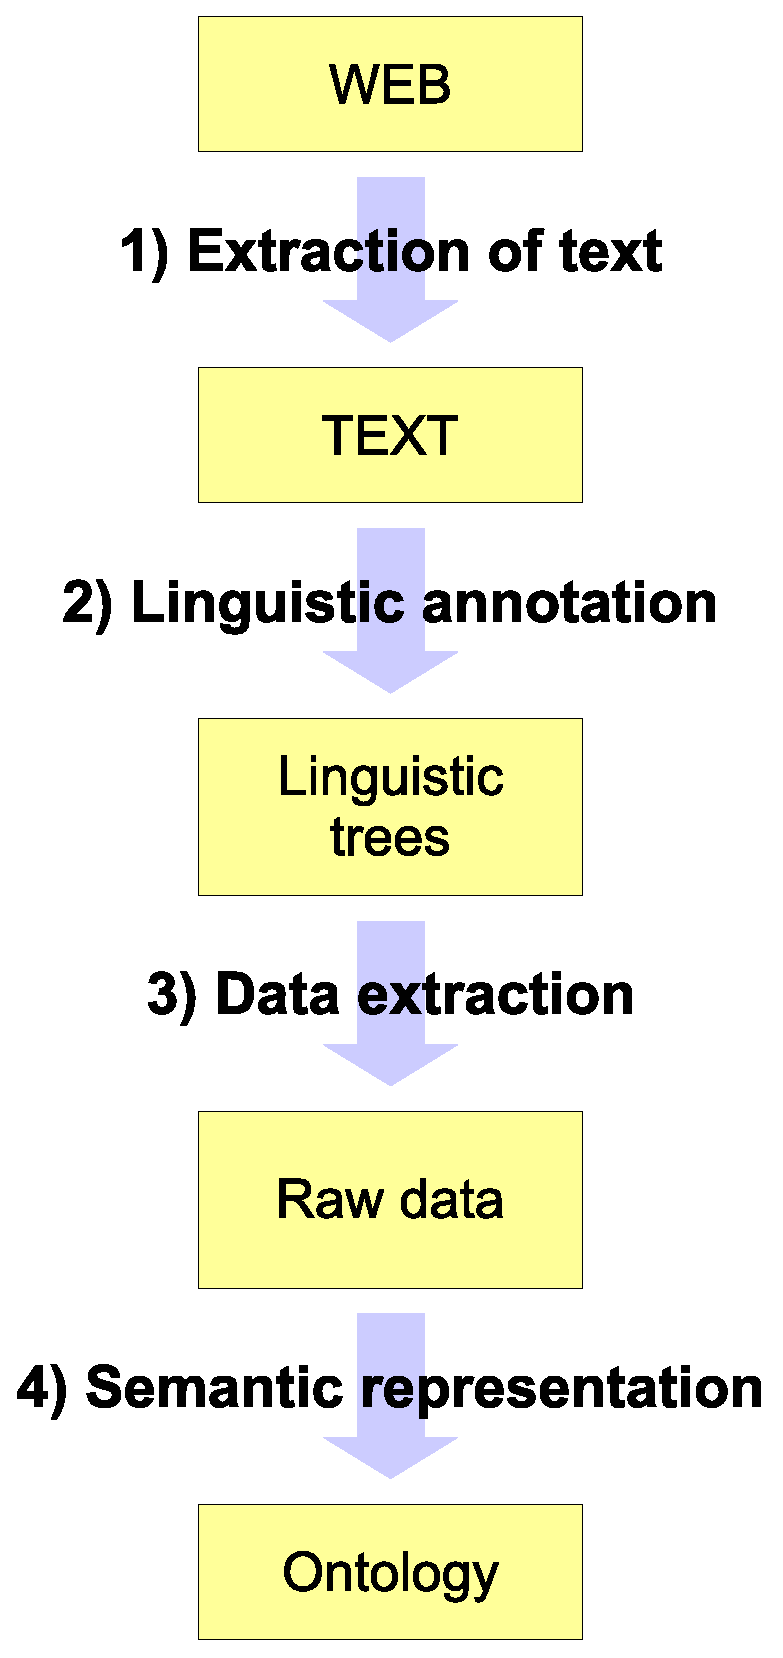
\includegraphics[height=0.8\vsize]{img/AP_schema1_en}
\column{.7\textwidth}
\begin{enumerate}
\item Extraction of text
\begin{itemize}
	\item Using \alert{RSS feed} to download pages.
	\item \alert{Regular expression} to extract text.
\end{itemize}
\item Linguistic annotation
\begin{itemize}
	\item Using \alert{chain} of 6 linguistic tools\\(see on next slides).
\end{itemize}
%In this phase the linguistic annotators process the extracted text and produce corresponding set of dependency trees representing the deep syntactic structure of individual sentences. We have used the linguistic tools described in the section~\ref{sec:ling_tools} for this task.
\item Data extraction
\begin{itemize}
	\item Exploitation of linguistic trees.
	\item Using \alert{extraction rules}.	
\end{itemize}
%We use the structure of tectogrammatic (i.e. deep syntactic) dependency trees to extract relevant data. 
\item Semantic representation of data
\begin{itemize}
	\item Ontology needed.
	\item Semantic interpretation of rules.
	\item Far from finished in current state.
\end{itemize}
%This phase consists of quite simple data transformation or conversion to the desired ontology format. But it is quite important to choose suitable ontology that will properly represent semantics of the data. We have not implemented this phase yet.
\end{enumerate}
\end{columns}
\end{frame}



\subsection{Linguistics we have used.}

\begin{frame}{Layers of linguistic annotation in PDT}
\begin{columns}
\column{.5\textwidth}
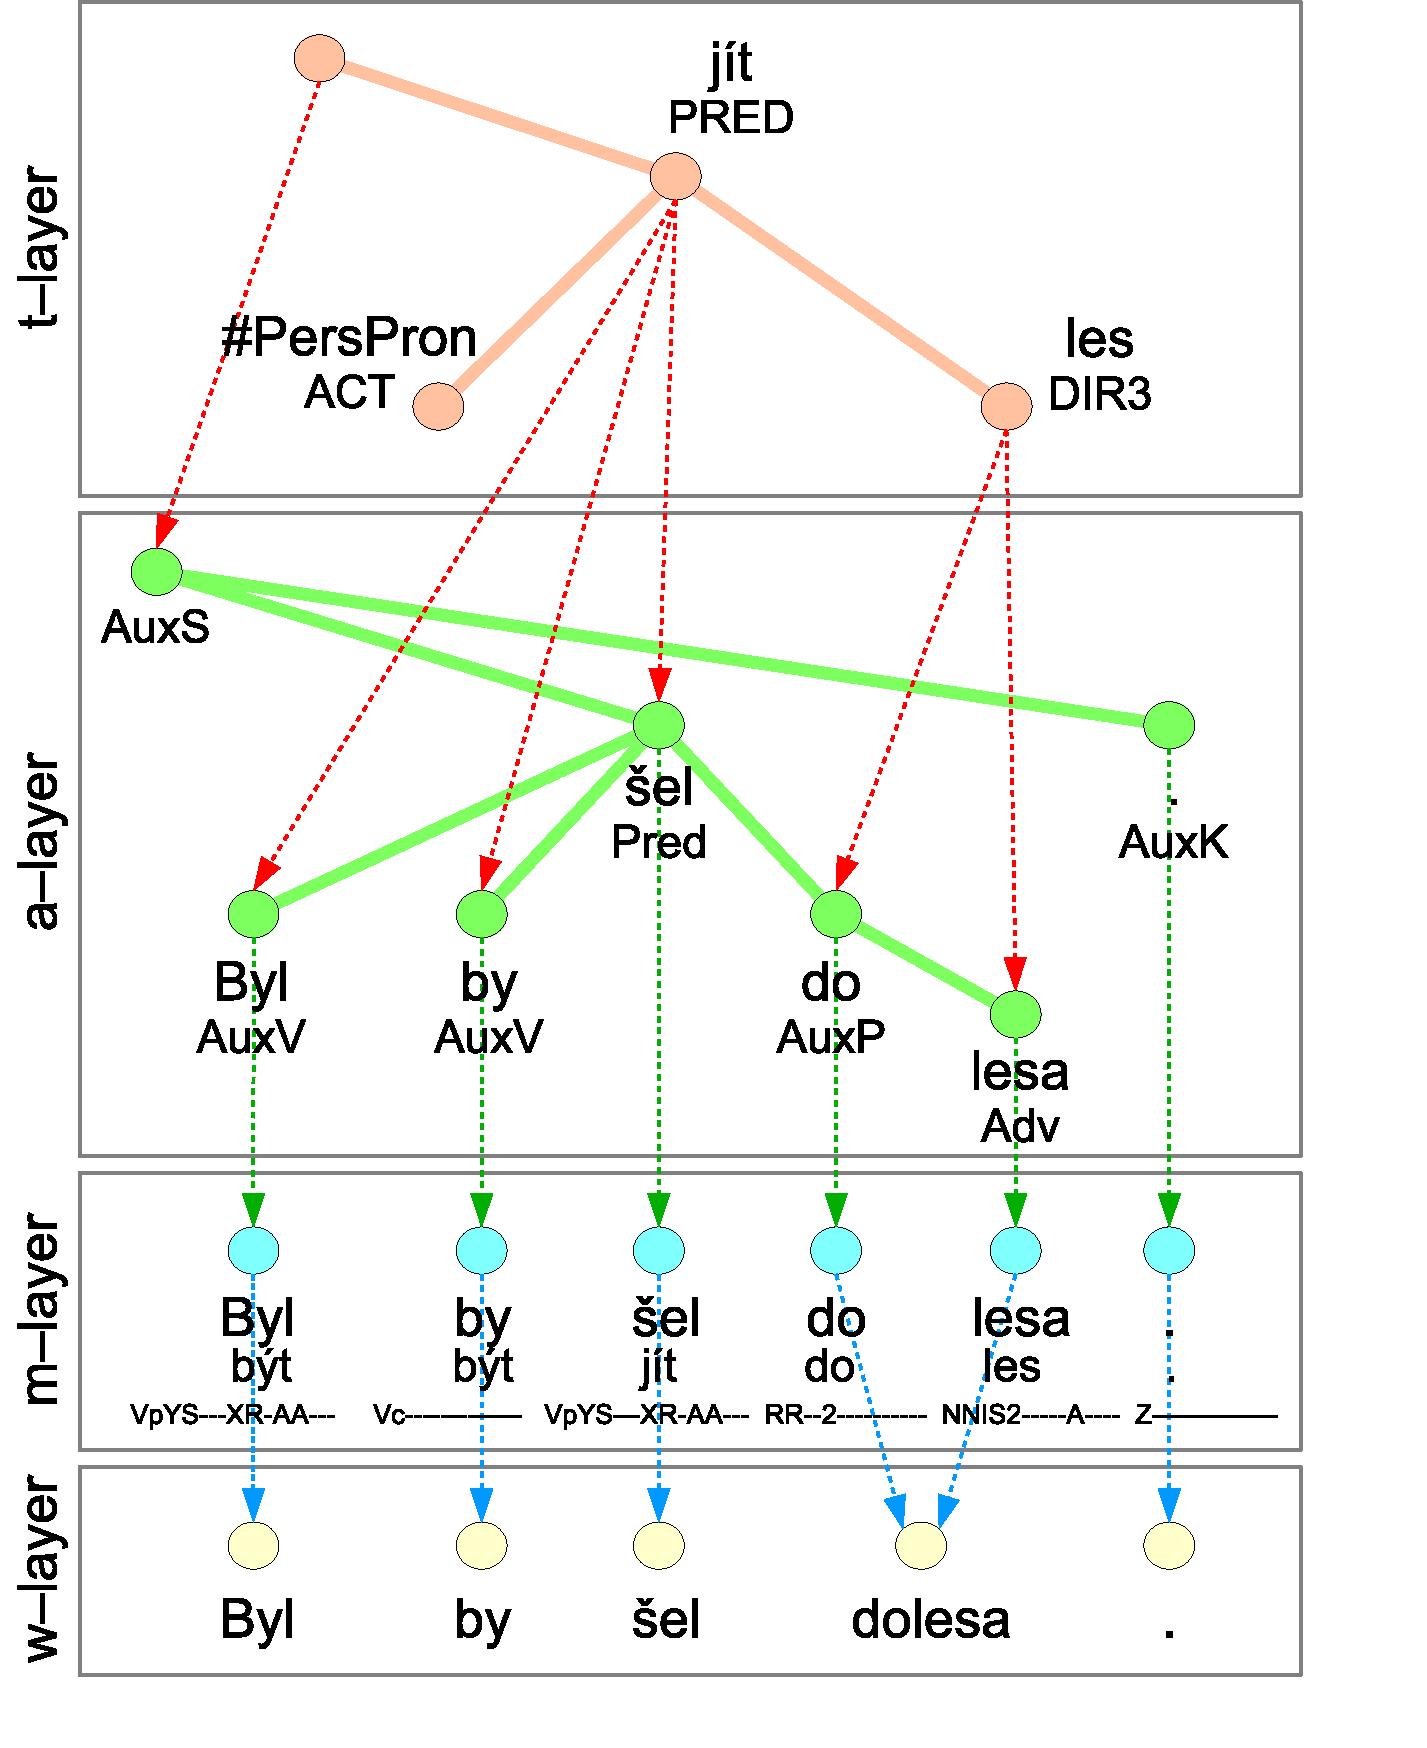
\includegraphics[height=0.9\vsize]{img/PDT_layers}
\column{.5\textwidth}
\begin{itemize}
	\item Tectogrammatical layer
	\item Analytical layer
	\item Morphological layer
\end{itemize}
\vspace{2cm}
\emph{Sentence:}
\medskip
\\Byl by �el dolesa.
\\He-was would went toforest.
\end{columns}
\end{frame}

\begin{frame}{Tools for machine linguistic annotation}
  \begin{block}{Available on the PDT 2.0 CD-ROM} %\footnote{\url{http://ufal.mff.cuni.cz/pdt2.0/}}
		\begin{enumerate}
			\item Segmentation and tokenization
			\item Morphological analysis
			\item Morphological tagging	
			\item Collins' parser -- Czech adaptation
			\item Analytical function assignment
		\end{enumerate}
  \end{block}  
	\begin{enumerate}
		\addtocounter{enumi}{5}
		\item Tectogrammatical analysis\\
		-- Developed by V�clav Klime�
	\end{enumerate}  
\end{frame}

\begin{frame}{Example of tectogrammatical tree}
\begin{columns}
\column{.5\textwidth}
\includegraphics[height=0.9\vsize]{img/DedVoj_tecto_tree}
\column{.5\textwidth}
\begin{itemize}
	\item Lemmas
	\item Functors
	\item Semantic parts of speech
\end{itemize}
\vspace{0.7cm}
\emph{Sentence:}
\medskip
{\small
\\Ve zdemolovan�m trabantu na m�st� zem�eli dva mu�i -- 82let� senior a dal�� mu�, jeho� toto�nost zji��uj� policist�.
\medskip
\\Two men died on the spot in demolished trabant -- \dots }
\end{columns}
\end{frame}


\subsection{Domain of fire-department articles}

\begin{frame}{Example of the web-page with a report of a fire department}
\begin{columns}
\column{\textwidth}
\includegraphics[height=0.9\vsize]{img/DedVoj_article}
\end{columns}
\end{frame}

\begin{frame}{Domain of our experiments}
\begin{itemize}
	\item \alert{Fire-department articles}
	\item Published by The Ministry of Interior of the Czech Republic\footnote{\url{http://www.mvcr.cz/rss/regionhzs.html}}
	\item Processed more than 800 articles 
	\\from different regions of Czech Republic
	\item 1.2 MB of textual data
	\item Linguistic tools produced 10 MB of annotations,\\run time 3.5 hours
	\item Extracting information about \alert{injured and killed people}
	\item 470 matches of the extraction rule,\\200 numeric values of quantity (described later)
\end{itemize}
\end{frame}




\begin{frame}{Example of processed text}
\centerline{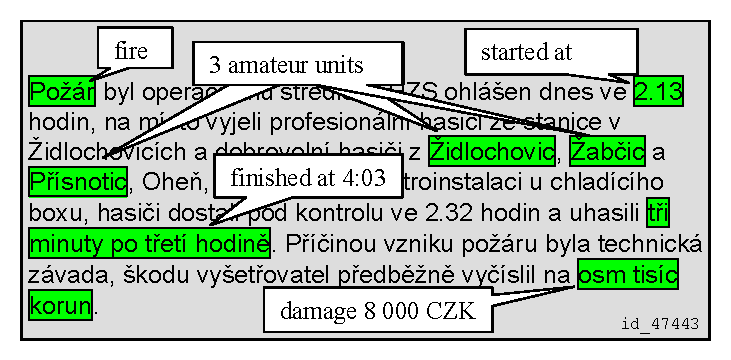
\includegraphics[height=0.5\vsize]{img/message}}
\bigskip
\begin{itemize}
	\item Information to be extracted is decorated.
	\item See the last sentence on the \alert{next slide}.
\end{itemize}
\end{frame}

\begin{frame}{Example of a linguistic tree}
\centerline{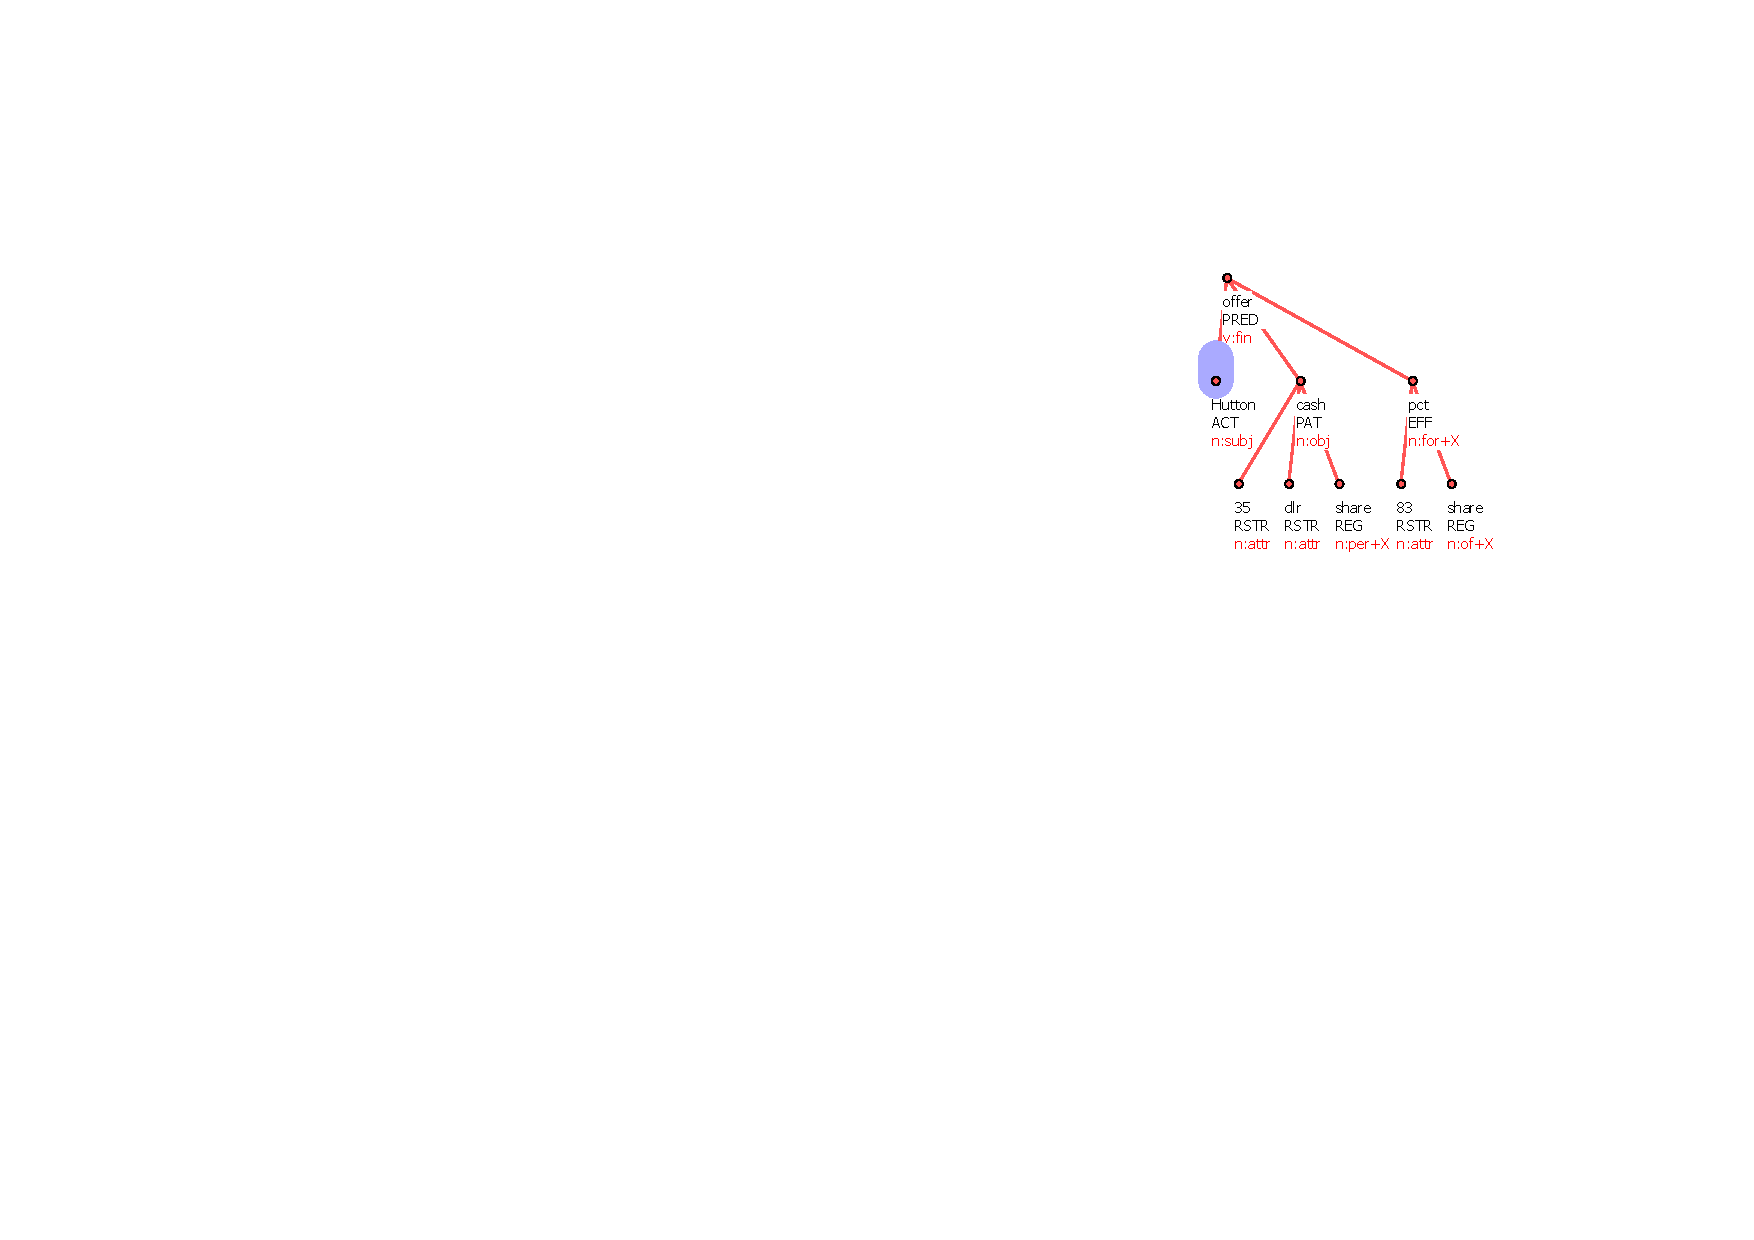
\includegraphics[height=0.7\vsize]{img/tree}}
\begin{itemize}
	\item Our IE method uses \alert{tree queries} (tree patterns)
\end{itemize}
\end{frame}

\section{Our Information Extraction Method}
\frame{\tableofcontents[currentsection]}
\subsection{Manually created rules}

\begin{frame}[plain]
\begin{columns}
\column{.67\textwidth}
%\centerline{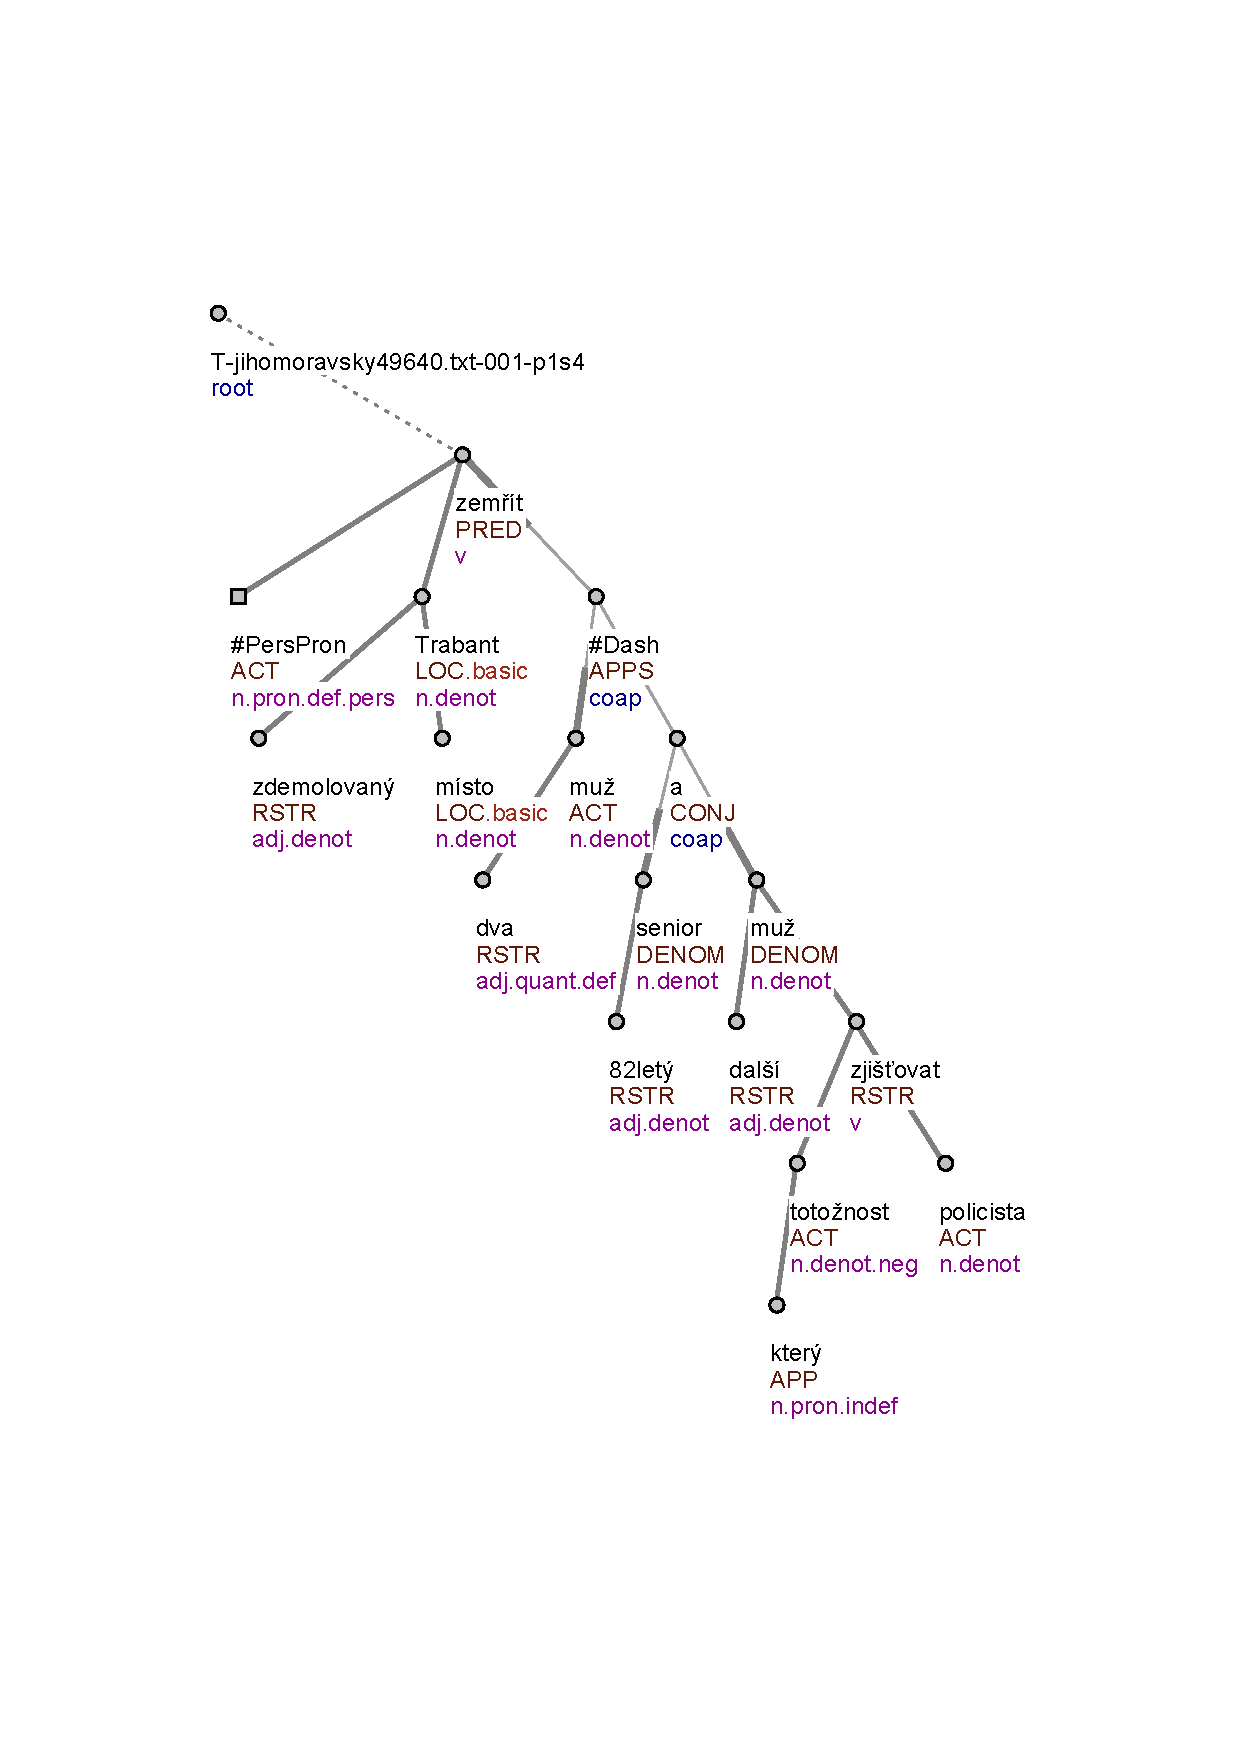
\includegraphics[height=1.1\vsize,width=\hsize]{img/TectogramaticalTree}}
\centerline{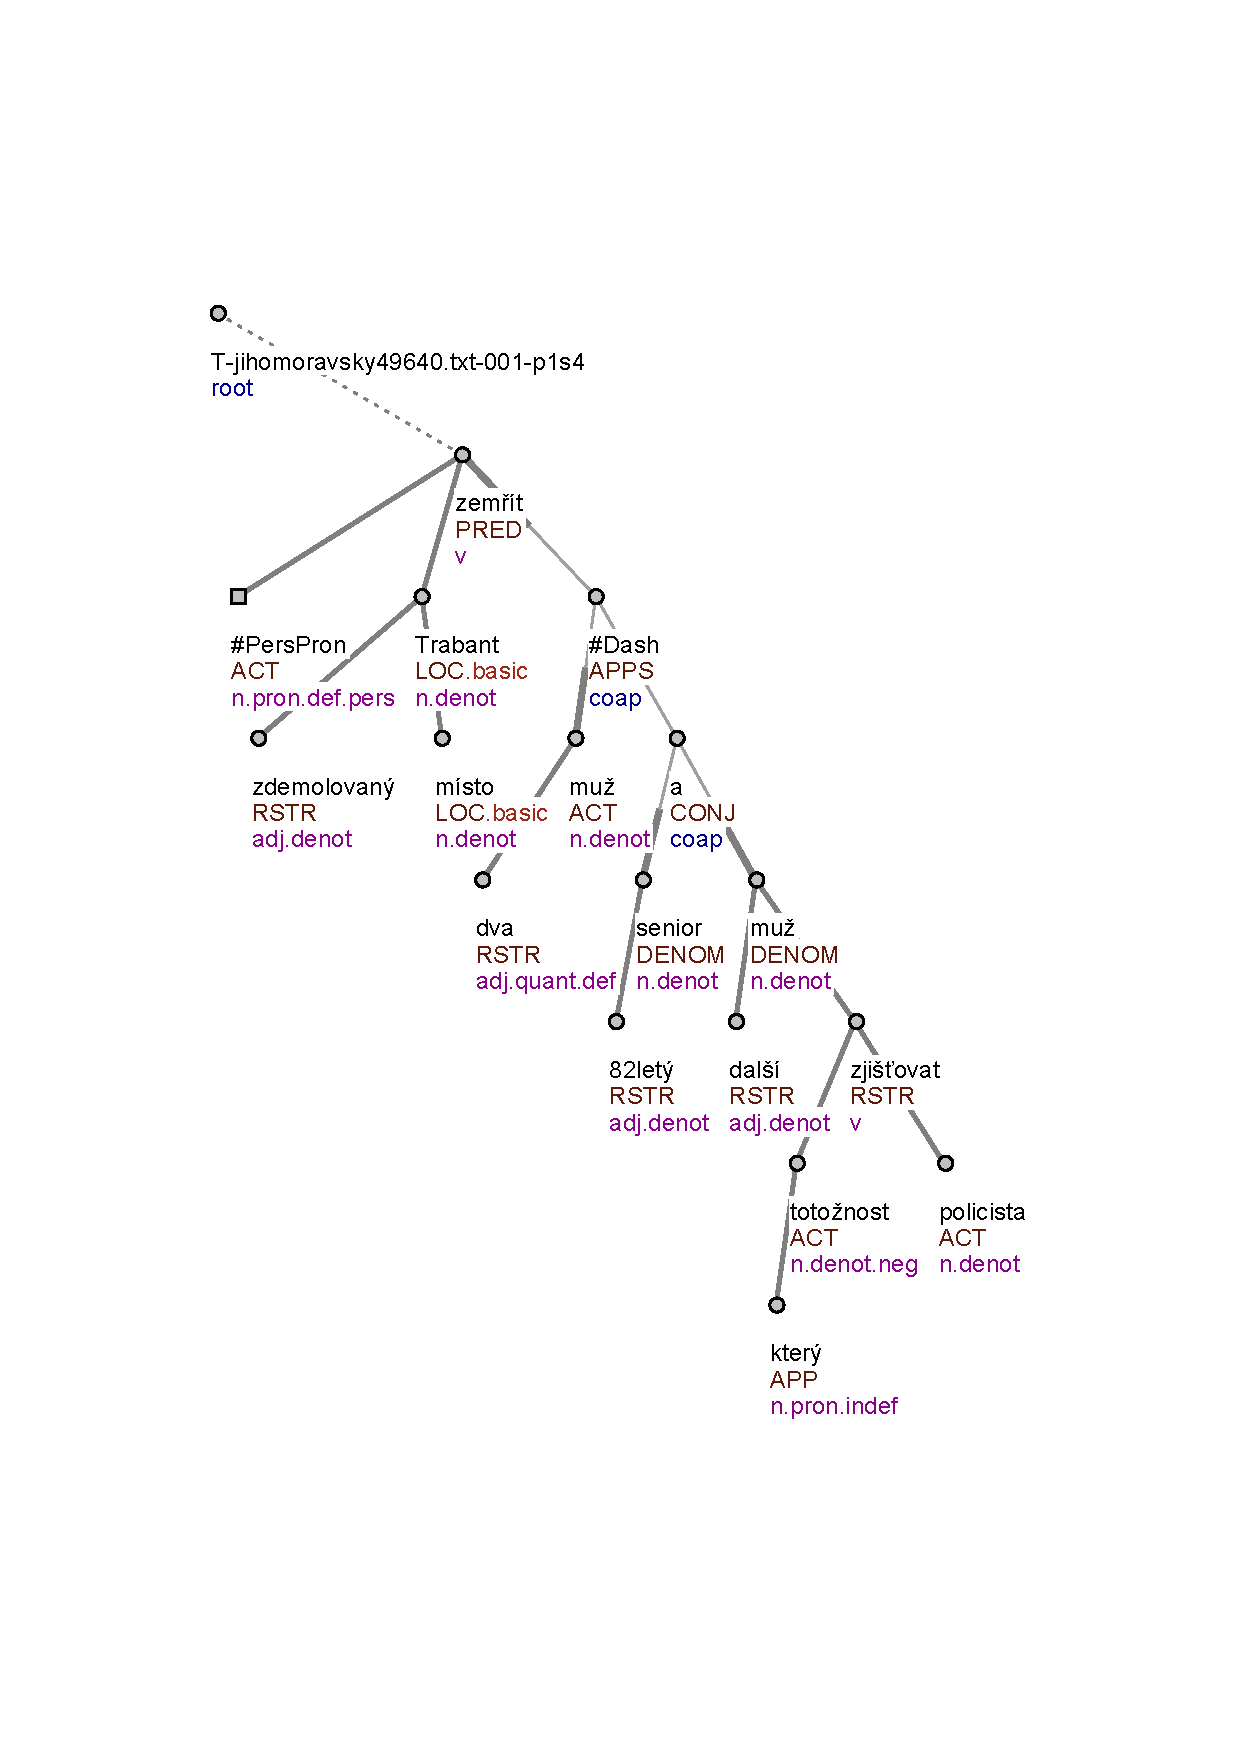
\includegraphics[height=1.1\vsize]{img/TectogramaticalTree}}
\column{.33\textwidth}
\begin{itemize}
	\item How to extract the information about \alert{two dead} people?
\end{itemize}
\vspace{2cm}
\end{columns}
\end{frame}

\begin{frame}{Extraction rules -- Netgraph queries}
\begin{center}
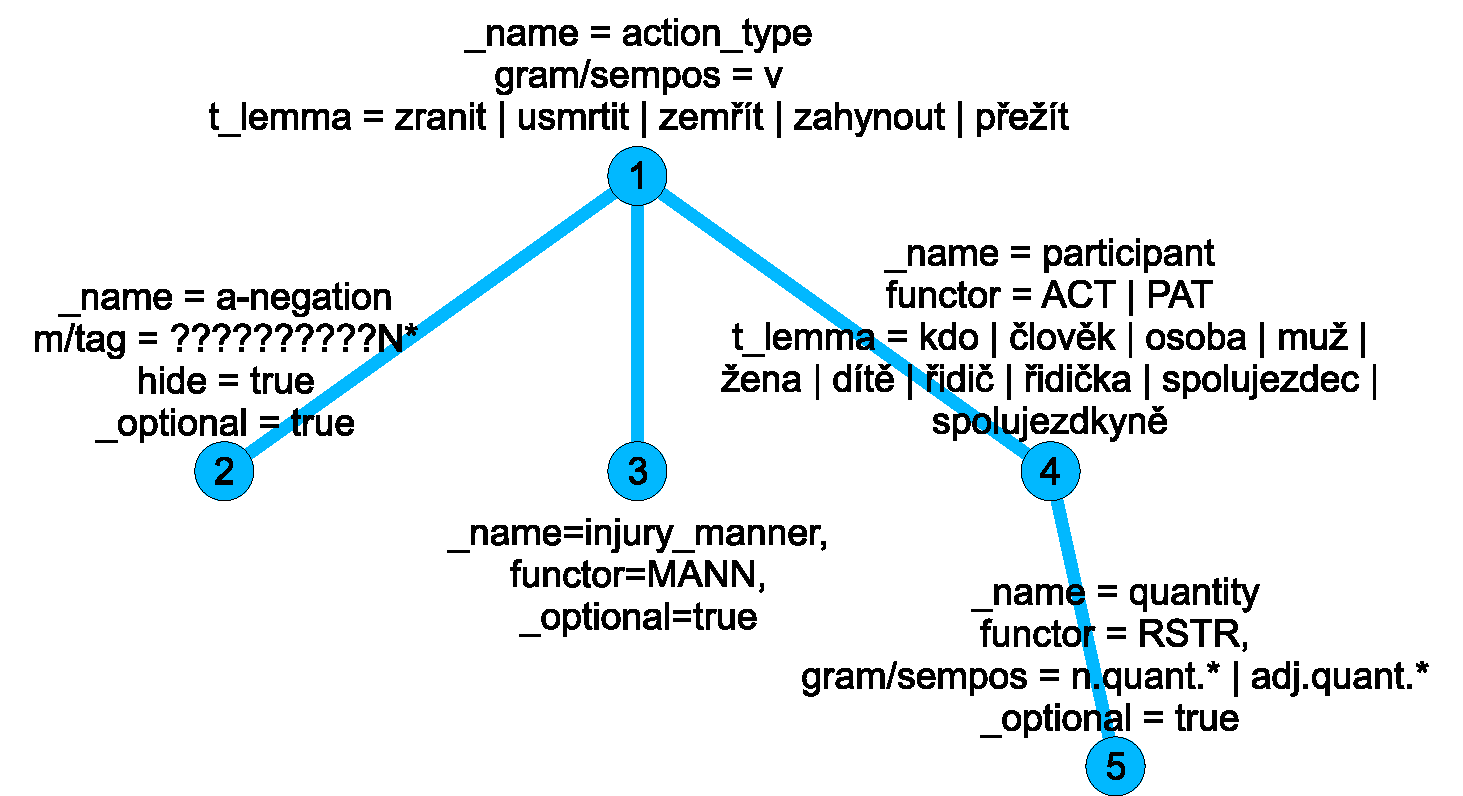
\includegraphics[height=0.6\vsize]{img/extract_patern}
\end{center}
\begin{itemize}
	\item Tree patterns on \alert{shape} and \alert{nodes} (on node attributes).
	\item Evaluation gives \alert{actual matches} of particular nodes.
	\item \alert{Names} of nodes allow use of references.
\end{itemize}
\end{frame}


\begin{frame}{Raw data extraction output}
%\begin{center}
\centerline{\includegraphics[height=0.8\vsize]{img/DedVoj_OutputQueryMatches}}
%\end{center}

{\scriptsize
\textbf{SELECT} \alert{action\_type}.t\_lemma, \alert{a-negation}.m\/tag, 
\alert{injury\_manner}.t\_lemma, \alert{participant}.t\_lemma,
\alert{quantity}.t\_lemma \textbf{FROM} \emph{***extraction rule***} 
}
\end{frame}


\begin{frame}{Semantic interpretation of extraction rules}
\begin{center}
\includegraphics[width=\hsize]{img/DedVoj_semantic_interpretation}
\end{center}
\begin{itemize}
	\item Determines how particular values of attributes are used.
	\item Gives semantics to extraction rule.
	\item Gives semantics to extracted data.
\end{itemize}
\end{frame}

\begin{frame}{Semantic data output}
\includegraphics[width=\hsize]{img/DedVoj_instances}
\bigskip
\begin{itemize}
	\item Two instances of two ontology classes.
\end{itemize}
\end{frame}


\begin{frame}{The experimental ontology}
\begin{columns}
\column{.45\textwidth}
\includegraphics[height=0.6\vsize]{img/DedVoj_classes}
\column{.55\textwidth}
\begin{itemize}
	\item Two \alert{classes}	
		\begin{itemize}
			\item Incident and Participant
		\end{itemize}
	\item One \alert{object property} relation
		\begin{itemize}
			\item hasParticipant
		\end{itemize}
	\item Five \alert{datatype property} relations
		\begin{itemize}
			\item actionManner \\(light or heavy injury)
			\item negation
			\item actionType \\(injury or death)
			\item participantType \\(man, woman, driver, etc.)
			\item participantQuantity
		\end{itemize}
\end{itemize}
\end{columns}
\end{frame}

\begin{frame}{Design of extraction rules -- iterative process}
\begin{center}
\includegraphics[height=0.6\vsize]{img/DedVoj_coverge_tuning}
\end{center}
\begin{enumerate}
	\item \alert{Frequency analysis} $\rightarrow$ representative key-words.
	\item Investigating of matching trees $\rightarrow$ \alert{tuning} of tree query.
	\item \alert{Complexity} of the query $\cong$ complexity of extracted data.
\end{enumerate}
\end{frame}



\subsection{Learning of rules}
\frame{\tableofcontents[currentsubsection]}

\begin{frame}{Integration of ILP in our extraction process}
\begin{center}
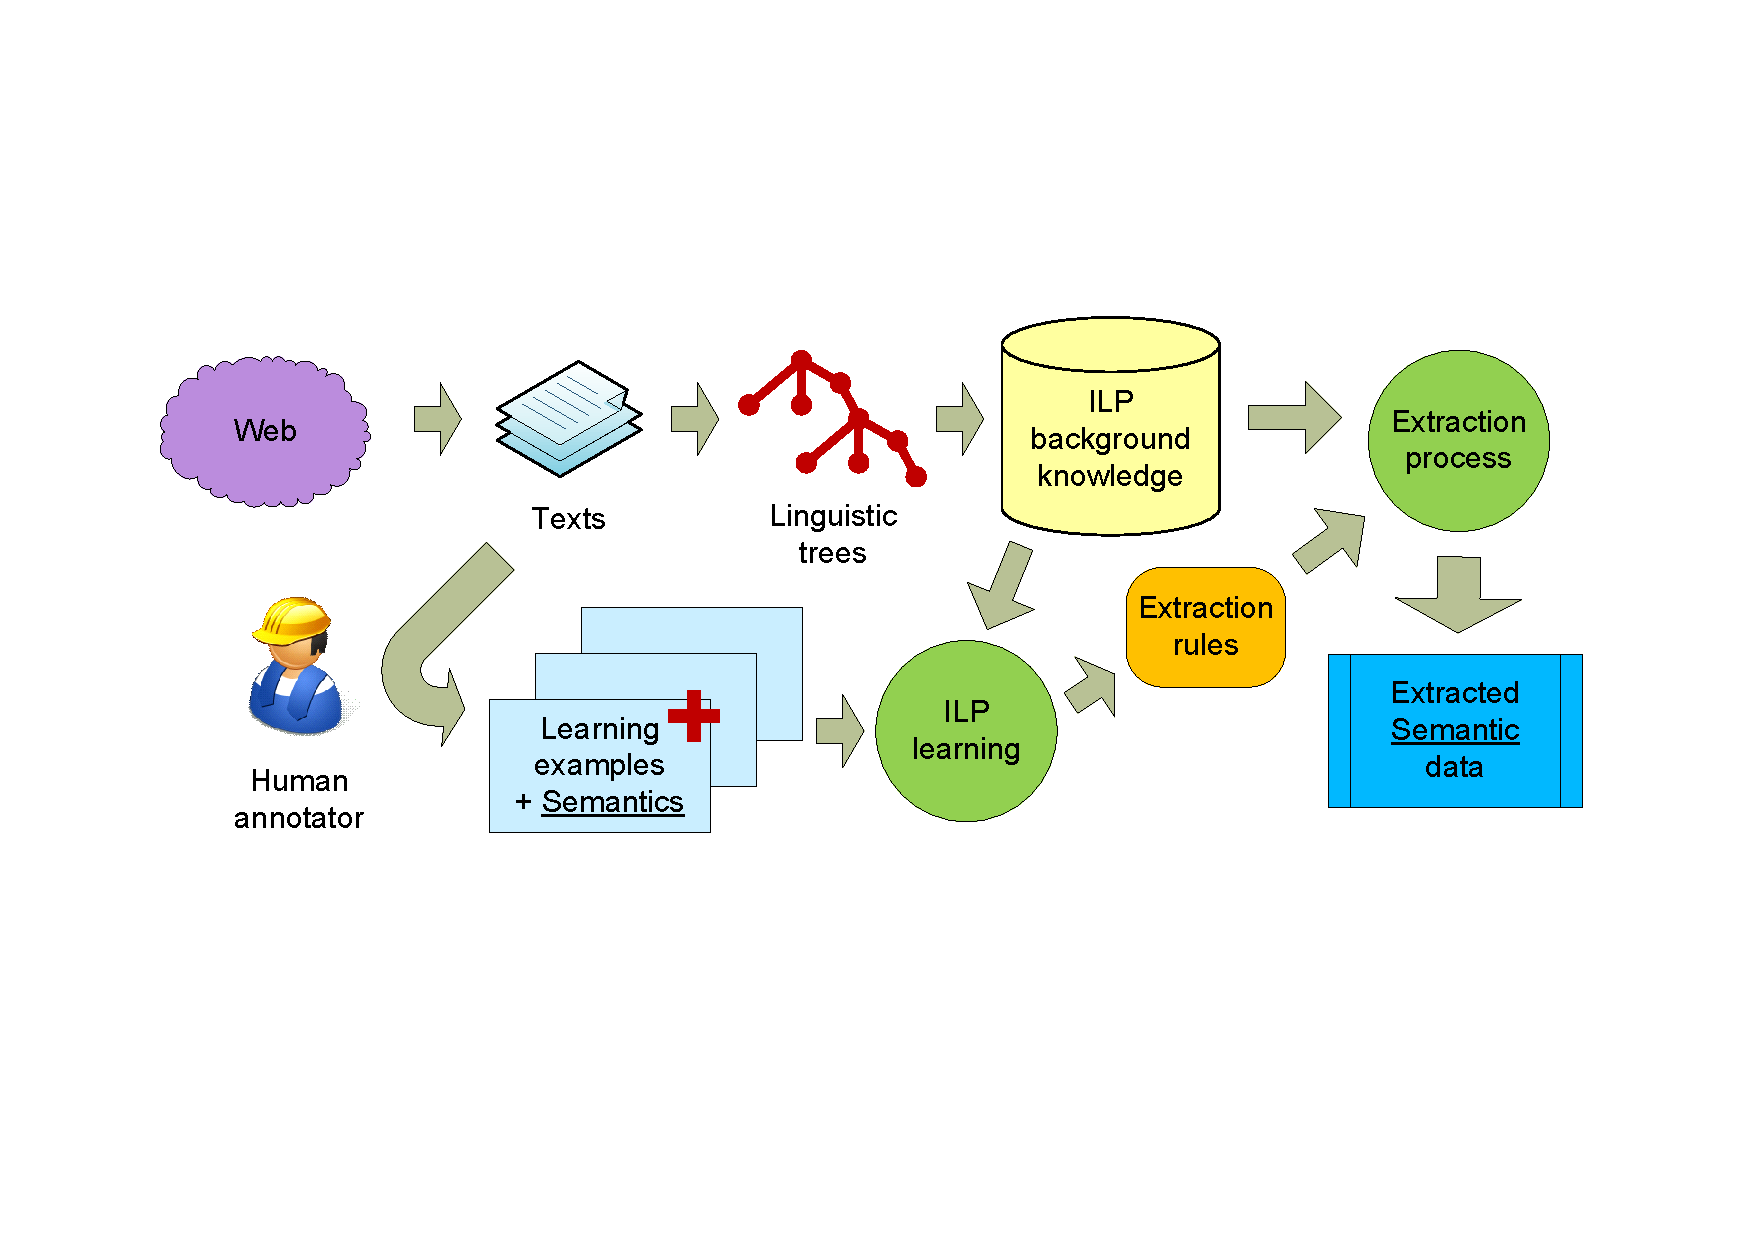
\includegraphics[width=\hsize]{img/DedVoj_ILP}
\end{center}
\begin{itemize}
	\item Transformation of trees to \alert{logic representation}. 
	\item Today: just \alert{first promising experiments}.
\end{itemize}
\end{frame}

\begin{frame}{Logic representation of linguistic trees}
\begin{columns}
\column{\textwidth}
\includegraphics[height=0.9\vsize]{img/DedVoj_LogicRepresentation}
\end{columns}
\end{frame}


\begin{frame}[fragile]{First promising results :-)}
\begin{example}
{\tiny \begin{verbatim}
contains_num_injured(A) :- t_lemma(A,1).
contains_num_injured(A) :- t_lemma(A,2).
contains_num_injured(A) :- t_lemma(A,23).
contains_num_injured(A) :- edge(A,B), m_form(B,jeden).
contains_num_injured(A) :- edge(A,B), m_tag(B,cn_s1__________).
contains_num_injured(A) :- edge(B,A), functor(B,conj).
contains_num_injured(A) :- edge(B,A), t_lemma(B,dite).
contains_num_injured(A) :- edge(B,A), t_lemma(B,muz).
contains_num_injured(A) :- edge(B,A), edge(B,C), m_tag14(C,1).
contains_num_injured(A) :- edge(B,A), edge(B,C), t_lemma(C,tezky).
contains_num_injured(A) :- edge(B,A), edge(B,C), t_lemma(C,nasledek).
contains_num_injured(A) :- edge(A,B), edge(C,A), m_tag4(B,1), functor(C,pat).
contains_num_injured(A) :- edge(A,B), edge(C,A), functor(C,act), a_afun(B,sb).
contains_num_injured(A) :- edge(B,A), edge(C,B), edge(C,D), t_lemma(D,vloni).
contains_num_injured(A) :- edge(B,A), edge(C,B), t_lemma(B,osoba), t_lemma(C,zranit).
contains_num_injured(A) :- edge(B,A), edge(C,B), t_lemma(B,osoba), t_lemma(C,zemrit).
contains_num_injured(A) :- edge(B,A), edge(C,B), functor(B,act), edge(C,D),
                           a_afun(D,obj).
contains_num_injured(A) :- edge(B,A), edge(C,B), t_lemma(B,osoba), edge(C,D), edge(D,E),
                           functor(D,twhen).
contains_num_injured(A) :- edge(B,A), t_lemma(A,tri), edge(B,C), edge(D,B), edge(E,D),
                           m_tag2(C,m).
\end{verbatim}}
\end{example}
\end{frame}


\section{Fuzzy ILP}
\frame{\tableofcontents[currentsection]}

\subsection{Introd. example, theory, architecture and an experiment}

\begin{frame}[fragile]{ILP Example}
\begin{block}{Types of ground variables}
{\footnotesize\begin{verbatim}
animal(dog). animal(dolphin) ... animal(penguin).
class(mammal). class(fish). class(reptile). class(bird).
covering(hair). covering(none). covering(scales).
habitat(land). habitat(water). habitat(air).
\end{verbatim}}
\end{block}
\begin{block}{Background knowledge}
{\footnotesize\begin{verbatim}
has_covering(dog, hair). has_covering(crocodile, scales).
has_legs(dog,4). ... has_legs(penguin, 2). etc.
has_milk(dog). ... has_milk(platypus). etc.
homeothermic(dog). ... homeothermic(penguin). etc.
habitat(dog, land). ... habitat(penguin, water). etc.
has_eggs(platypus). ... has_eggs(eagle). etc.
has_gills(trout). ... has_gills(eel). etc.
\end{verbatim}}
\end{block}
\end{frame}

\begin{frame}[fragile]{ILP Example}
\begin{columns}
\column{.5\textwidth}
\begin{block}{Positive examples}
{\footnotesize\begin{verbatim}
class(lizard, reptile).
class(trout, fish).
class(bat, mammal).
\end{verbatim}}
\end{block}
\column{.5\textwidth}
\begin{block}{Negative examples}
{\footnotesize\begin{verbatim}
class(trout, mammal).
class(herring, mammal).
class(platypus, reptile).
\end{verbatim}}
\end{block}
\end{columns}
\bigskip
\begin{block}{Induced rules}
{\footnotesize\begin{verbatim}
class(A,reptile) :- has_covering(A,scales),
                    has_legs(A,4).
class(A,mammal) :- homeothermic(A), has_milk(A).
class(A,fish) :- has_legs(A,0), has_eggs(A).
class(A,reptile) :- has_covering(A,scales),
                    habitat(A,land).
class(A,bird) :- has_covering(A,feathers).
\end{verbatim}}
\end{block}
\end{frame}


\begin{frame}{Classical ILP and Fuzzy ILP principles}
\begin{itemize}
	\item Learning examples $E=P\cup N$ (Positive and Negative)
	\item Background knowledge $B$
	\item ILP task -- to find hypothesis $H$ such that:
\end{itemize}
$$
(\forall e\in P)(B\cup H\models e) \ \ \&\  \ (\forall n\in N)(B\cup H\not\models n).
$$
\vspace{0.5cm}
\begin{itemize}
	\item Fuzzy learning examples ${\mathcal E}:E\longrightarrow [0,1]$
	\item Fuzzy background knowledge ${\mathcal B}:B\longrightarrow [0,1]$
	\item Fuzzy ILP task -- to find hyp. ${\mathcal H}:H\longrightarrow [0,1]$ such that:
\end{itemize}
$$
(\forall e_1,e_2\in E)(\forall {\mathcal M})({\mathcal M}\models_f {\mathcal B}\cup {\mathcal H}) \ :\ 
{\mathcal E}(e_1)>{\mathcal E}(e_2)\Rightarrow \left\|e_1\right\|_{{\mathcal M}}\ge \left\|e_2\right\|_{{\mathcal M}}
$$
\end{frame}

\begin{frame}{Generalized Annotated Programs}
\begin{itemize}
	\item Fuzzy ILP is equivalent to Induction of Generalized Annotated Programs\footnote{See in S. Krajci, R. Lencses and P. Vojtas: ``A comparison of fuzzy and annotated logic programming'', Fuzzy Sets and Systems, vol.144, pp.173�192, 2004.}
	\item For implementation we use GAP or strictly speaking: \emph{Definite Logic Programs with monotonicity axioms} (also equivalent)
	\item Basic paradigm: deal with \alert{values} as with \alert{degrees}.
		\begin{itemize}
			\item We don't have to normalize values, they order is enough.			
		\end{itemize}
	\medskip
	\item For example with monotonicity axioms we can use rule:
\centerline{\texttt{serious(A, 4)} $\leftarrow$ \texttt{fatalities(A, 10).}}
and from the fact \texttt{fatalities(id\_123, 1000)} deduce
\centerline{\texttt{serious\_alt(id\_123, 4).}}
\end{itemize}
\end{frame}


\begin{frame}{Schema of the whole system}
\begin{columns}
\column{.45\textwidth}
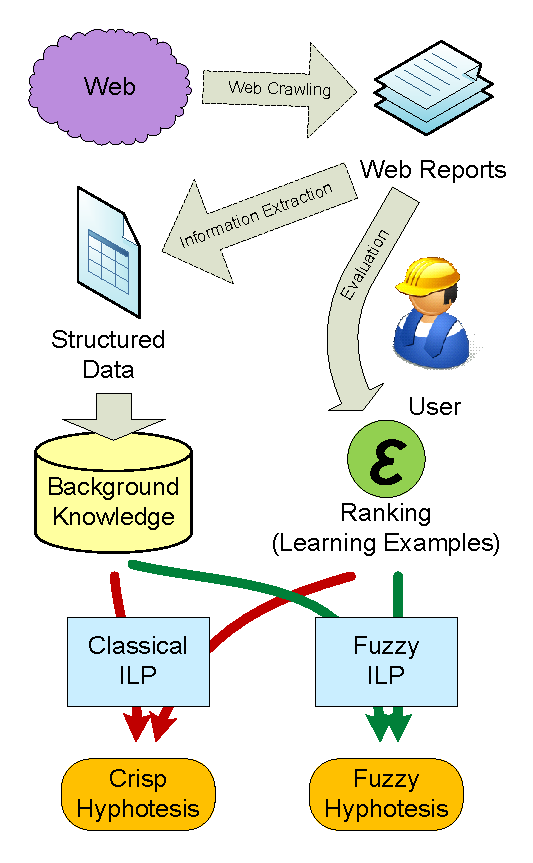
\includegraphics[height=0.9\vsize]{img/schema}
\column{.55\textwidth}
\begin{enumerate}
	\item Web Crawling
	\item Information Extraction and User Evaluation
	\item Logic representation
		\begin{itemize}
			\item Construction of \alert{background knowledge}
			\item Construction of \alert{learning examples}
		\end{itemize}
	\item ILP Learning
		\begin{itemize}
			\item Crisp
			\item Fuzzy
		\end{itemize}		
	\bigskip
	\item Comparison of results
\end{enumerate}
\end{columns}
\end{frame}


\begin{frame}{Accident attributes}
\begin{columns}
\column{.6\textwidth}
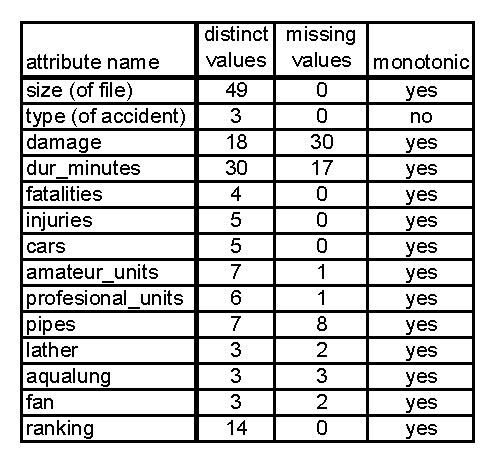
\includegraphics[height=0.75\vsize]{img/attributes_description}
\column{.4\textwidth}
\begin{itemize}
	\item Information that could be extracted.
	\item Missing values.
	\item Almost all attributes are \alert{numeric}.
		\begin{itemize}
			\item So \alert{monotonic}
			\item This will be used for ``fuzzyfication''
		\end{itemize}
	\item Artificial target attribute \alert{seriousness ranking}.
\end{itemize}
\end{columns}
\end{frame}


\begin{frame}{Histogram of the seriousness ranking attribute}
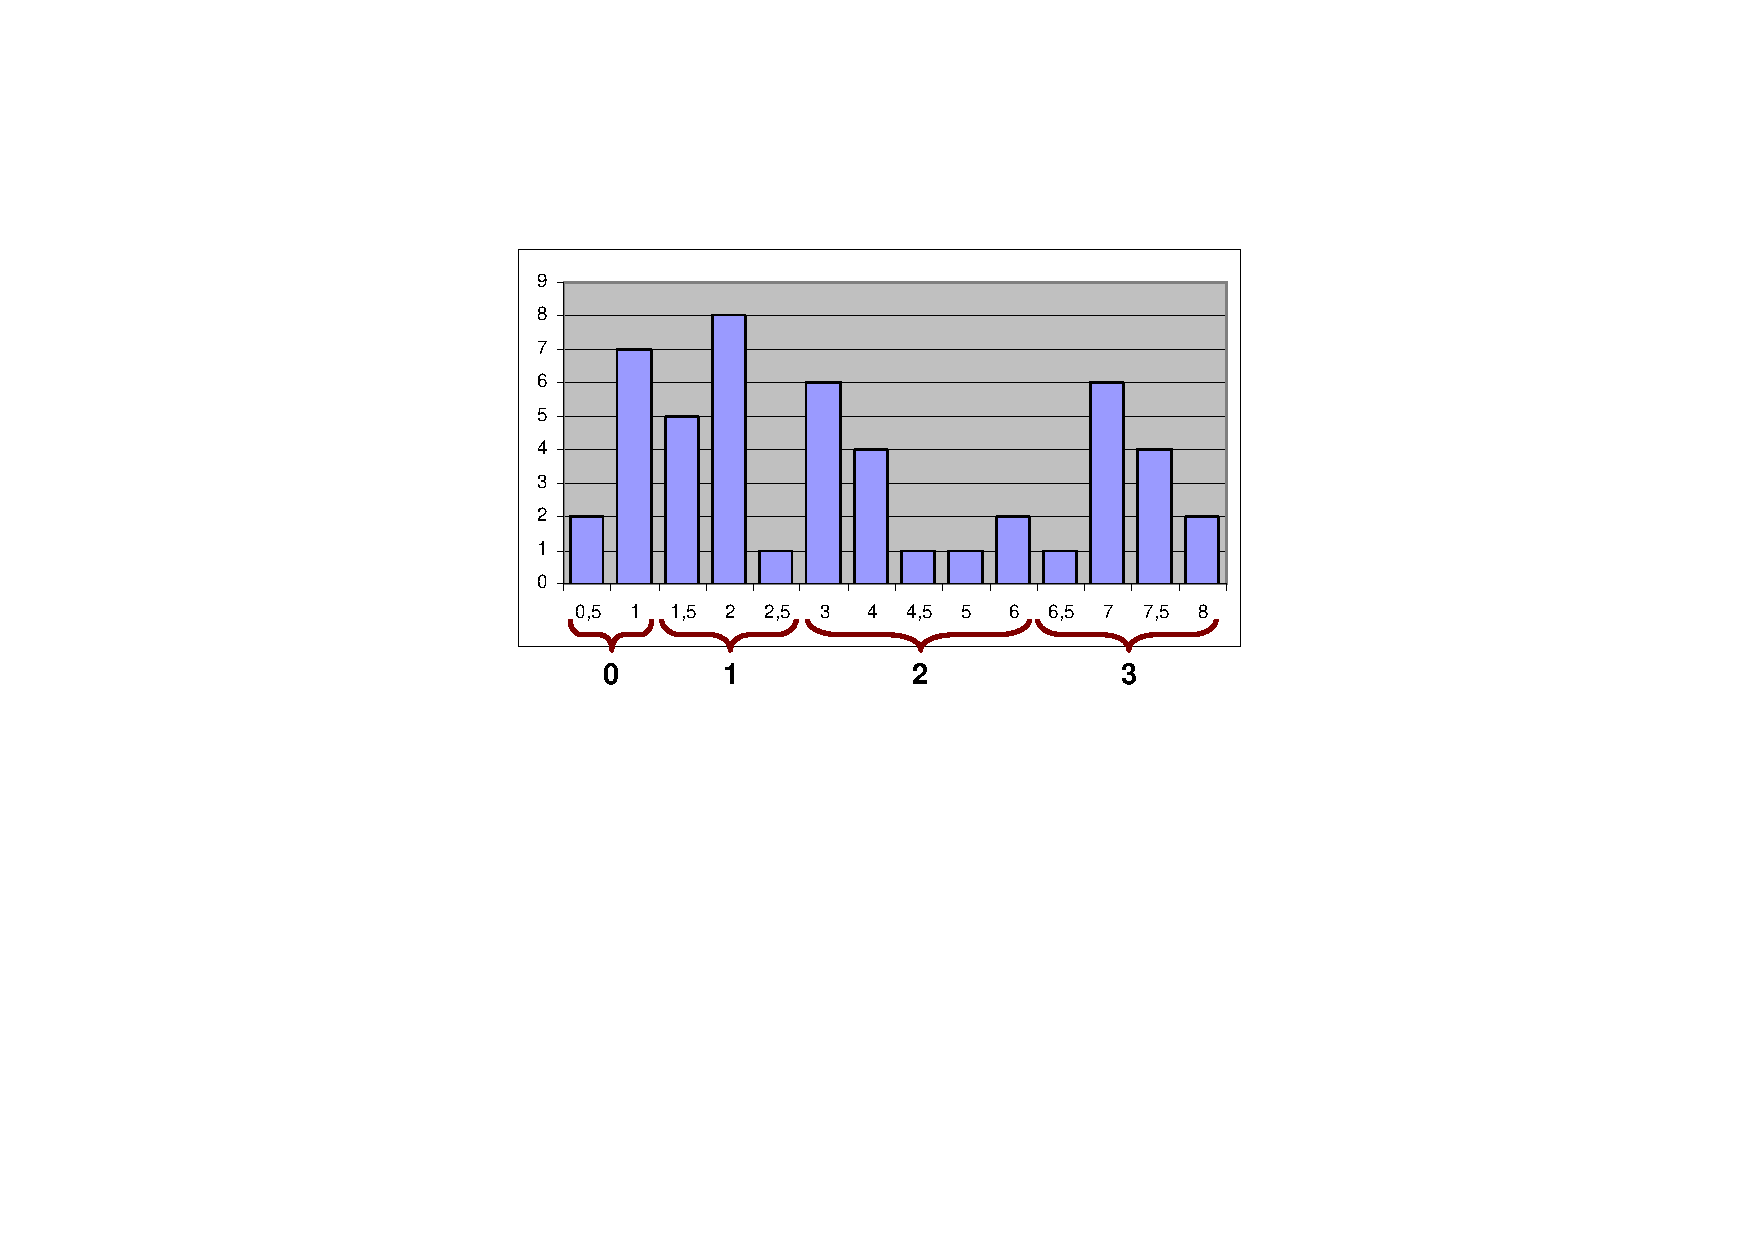
\includegraphics[width=0.9\hsize]{img/ranking_histogram}
\begin{itemize}
	\item 14 different values, range 0.5 -- 8
	\item Divided into four approximately \alert{equipotent groups}.
\end{itemize}
\end{frame}





\subsection{Fuzzy ILP Implementation}
\frame{\tableofcontents[currentsubsection]}

\begin{frame}{Essential difference between learning examples}
\begin{columns}
\column{.6\textwidth}
\setbeamercolor{block title}{bg=BrickRed}
\begin{block}{Crisp learning examples}
\centerline{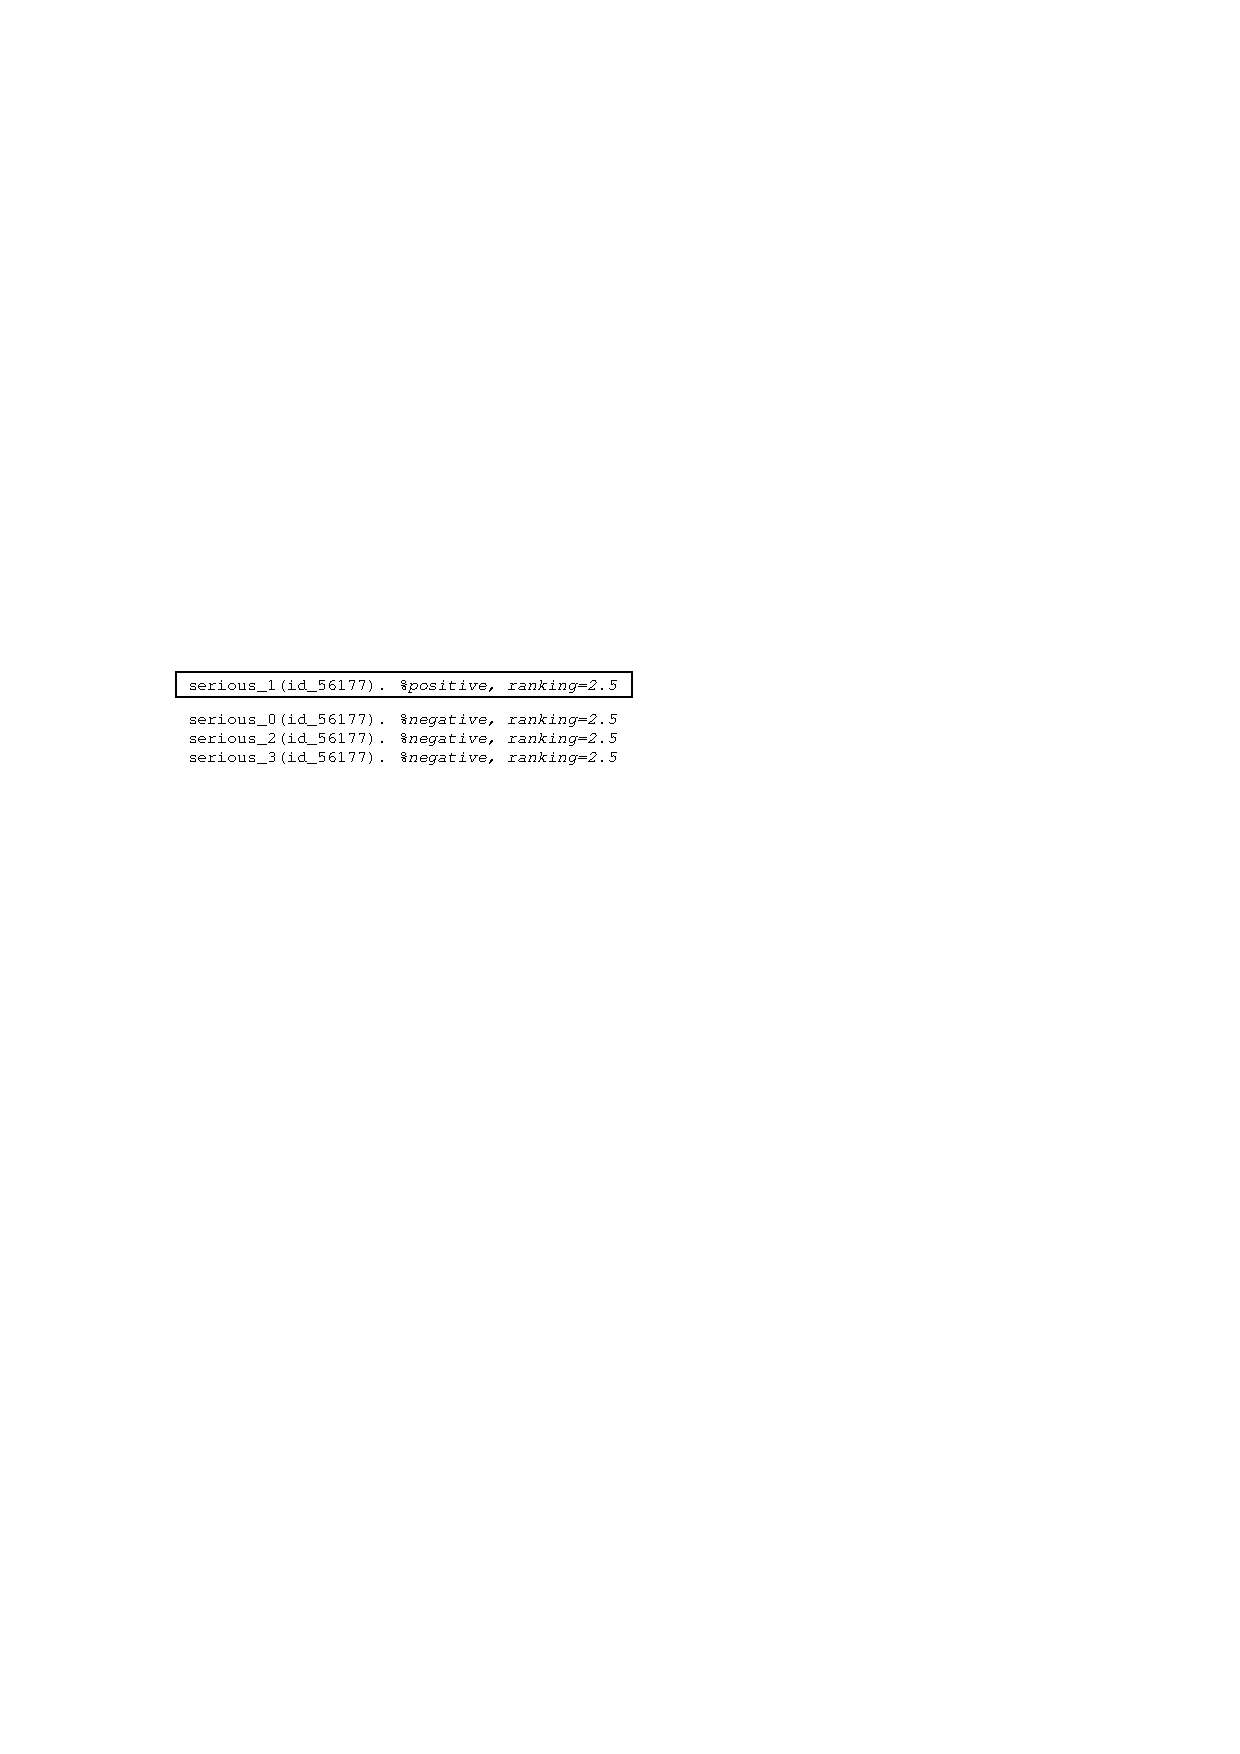
\includegraphics[width=\hsize]{img/examples_nonmonot}}
\end{block}
\bigskip
\setbeamercolor{block title}{bg=OliveGreen}
\begin{block}{Monotonized learning examples}
\centerline{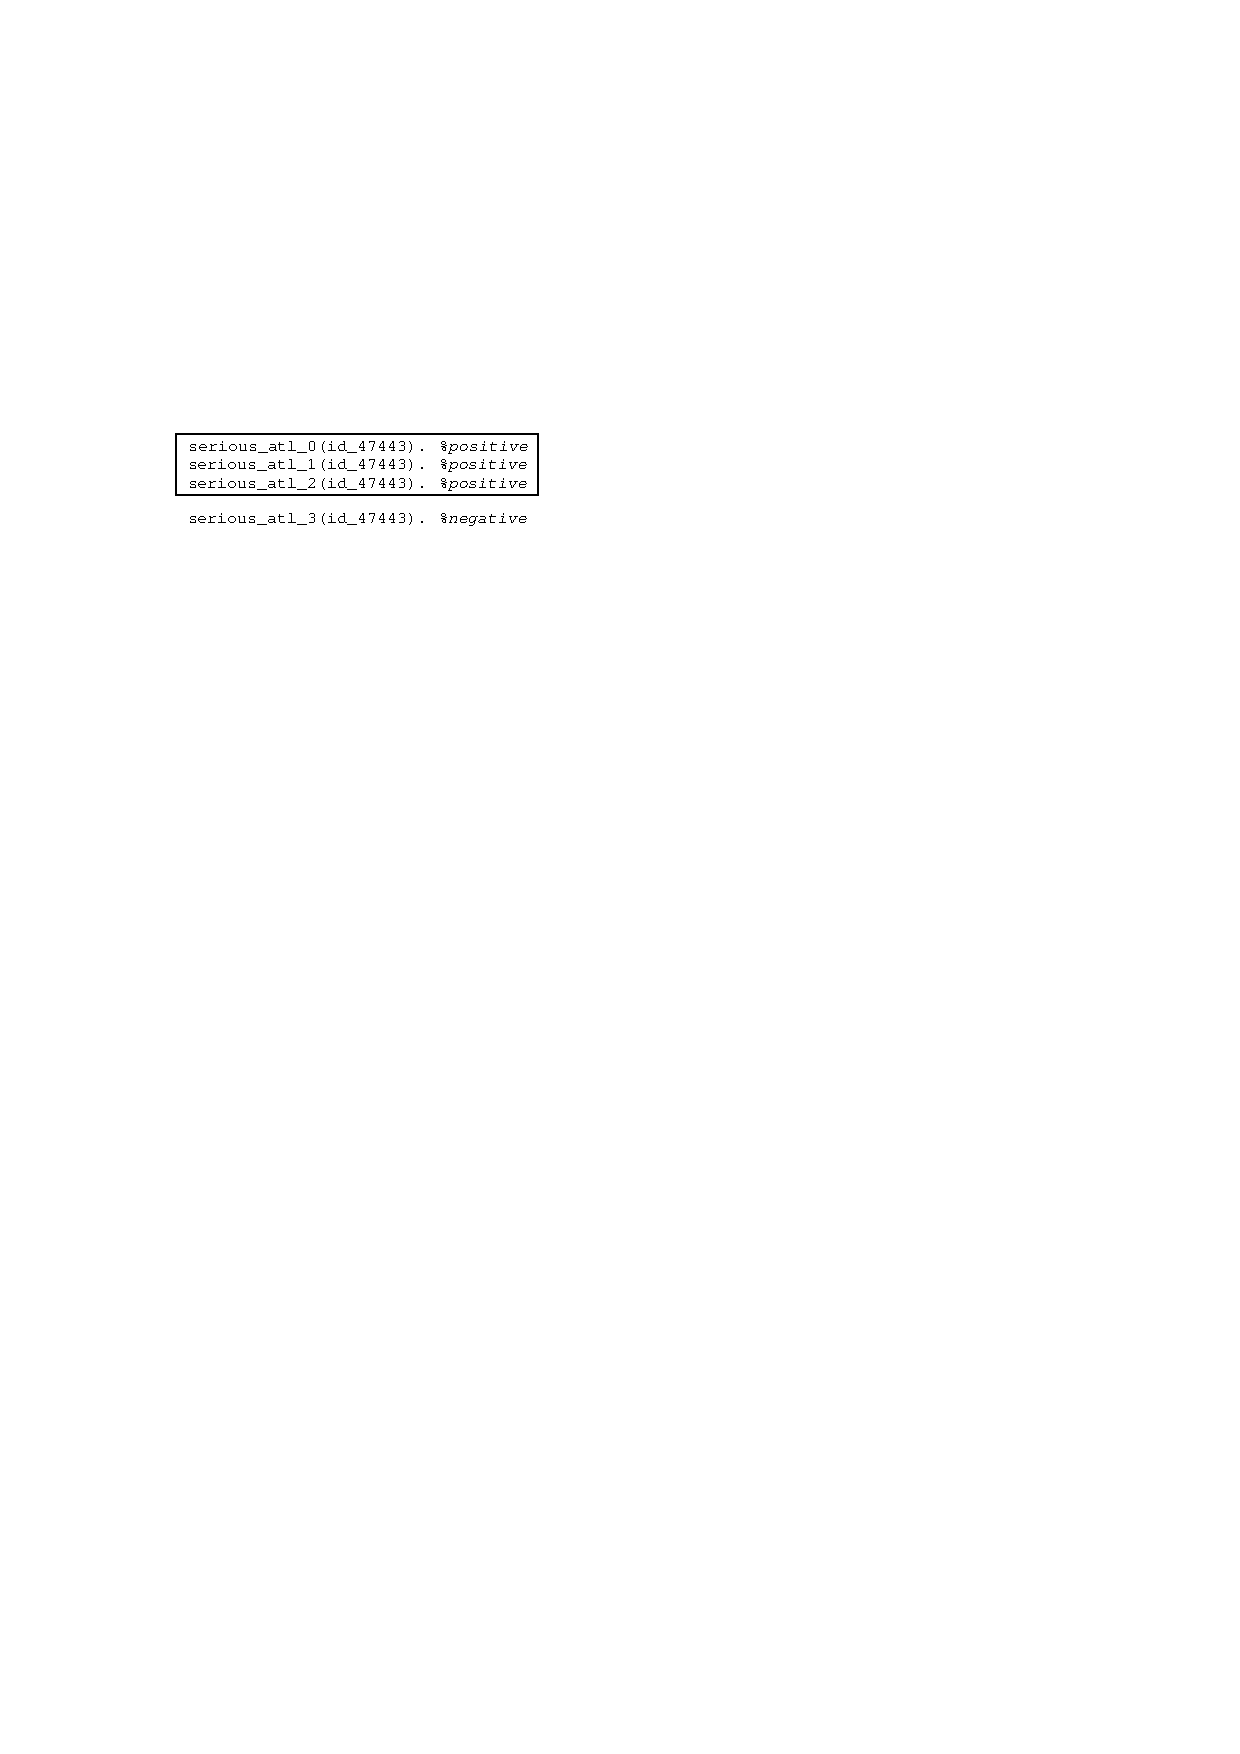
\includegraphics[width=\hsize]{img/examples_monot}}
\end{block}
\column{.4\textwidth}
For one evidence (occurrence):
	\bigskip
\begin{itemize}
	\item Crisp:\\
	Always \alert{one} positive and \alert{three} negative learning examples
	\bigskip
	\item Monotonized:\\
	\alert{Up to the observed degree} positive,\\the rest negative.
\end{itemize}
\end{columns}
\end{frame}


\begin{frame}{Monotonization of attributes}
\definecolor{MyBrown}{rgb}{0.5,0.5,0}
\setbeamercolor{block title}{bg=MyBrown}
\begin{block}{damage $\rightarrow$ damage\_atl}
\centerline{
\includegraphics[width=0.73\hsize]{img/attribute_monotonisation}}
\end{block}
\bigskip
\begin{itemize}
	\item We infer all lower values as sufficient.
	\item Treatment of unknown values.
	\item Negation as failure.
\end{itemize}
\end{frame}

\subsection{Evaluation and Conclusion}

\begin{frame}[plain]%{Crisp \& monotonized hypothesis}
\begin{columns}
\column{.67\textwidth}
\centerline{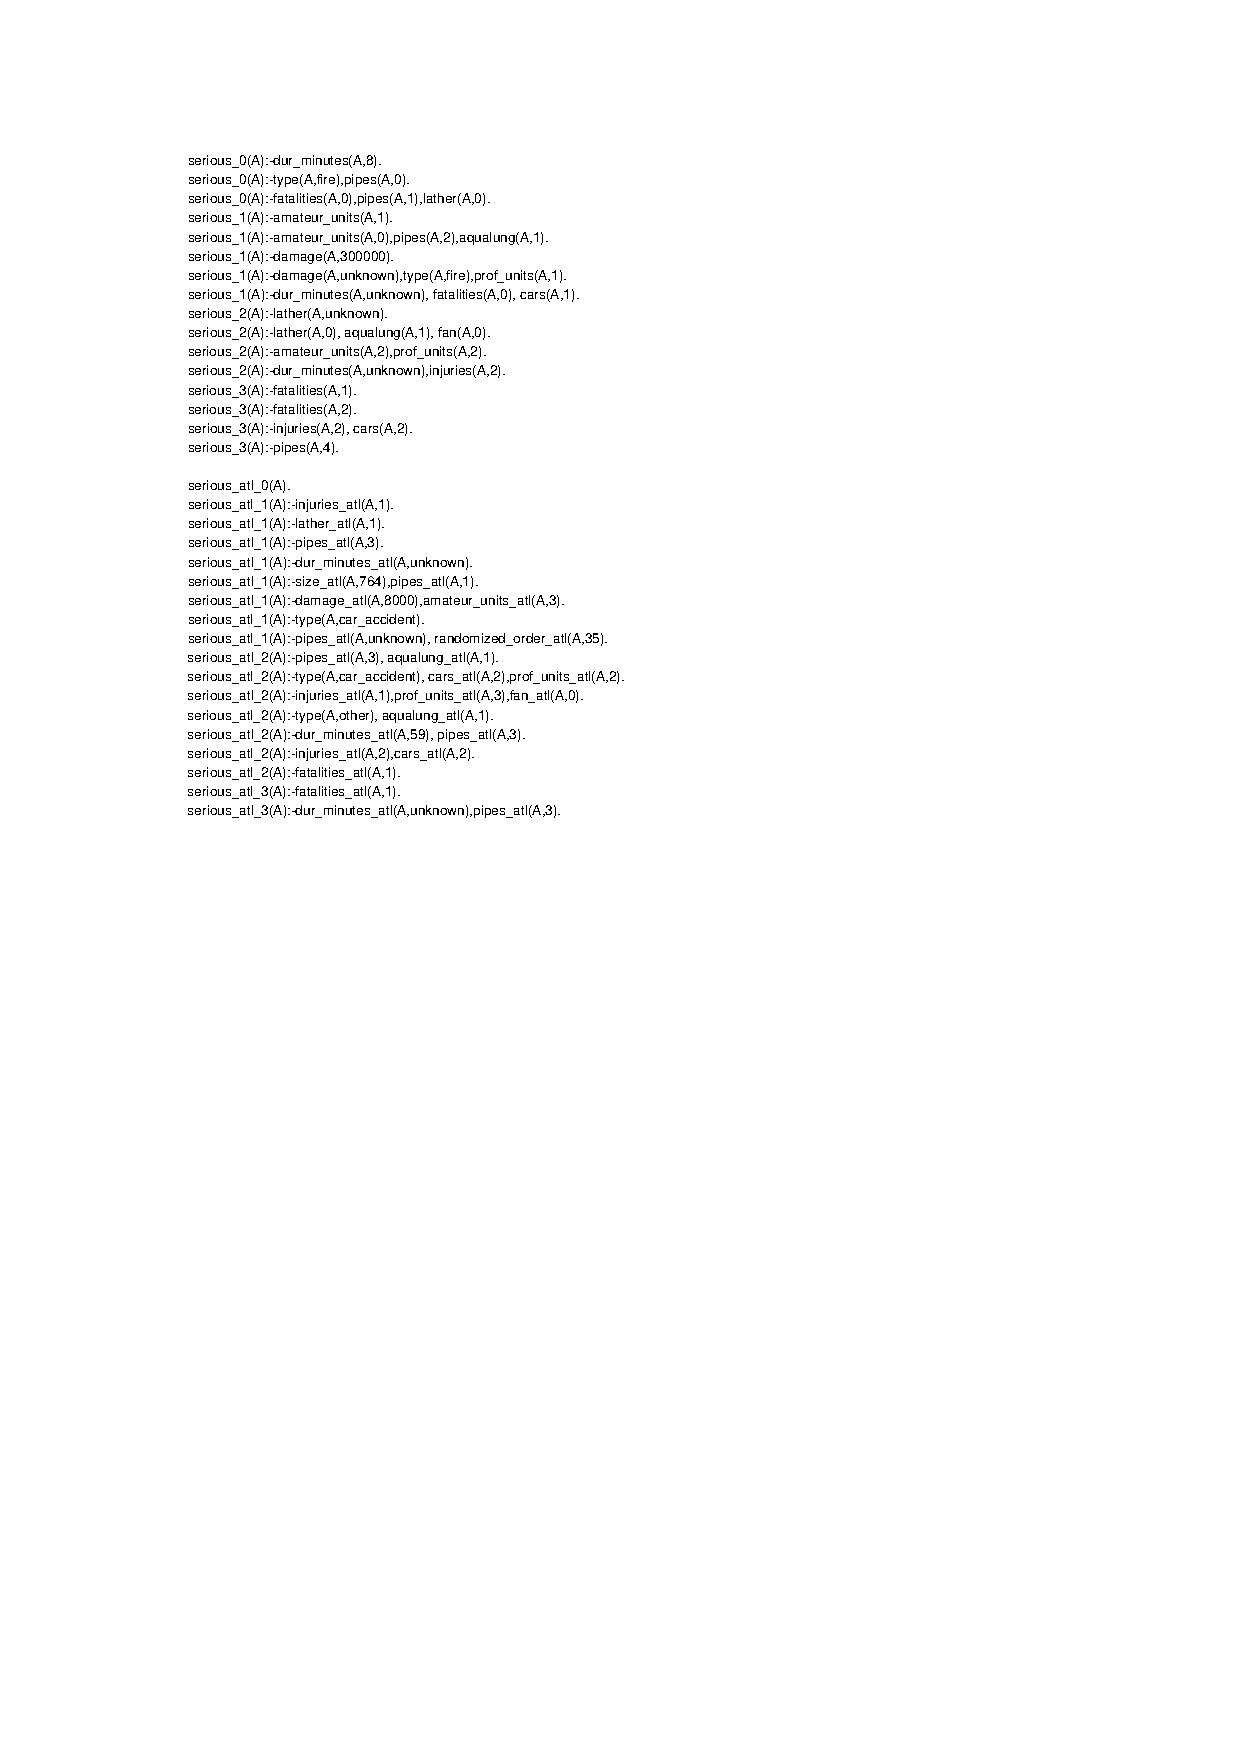
\includegraphics[height=1.1\vsize,width=\hsize]{img/rules}}
\column{.33\textwidth}
\begin{itemize}
	\item Crisp hypothesis
\vspace{3cm}
	\item Monotonized hypothesis	
	\begin{itemize}
		\item Monotonicity axioms
		\item Monotonized learning examples
	\end{itemize}
\end{itemize}
\vspace{2cm}
\end{columns}
\end{frame}

\begin{frame}{Evaluation and Comparison of Results}
\centerline{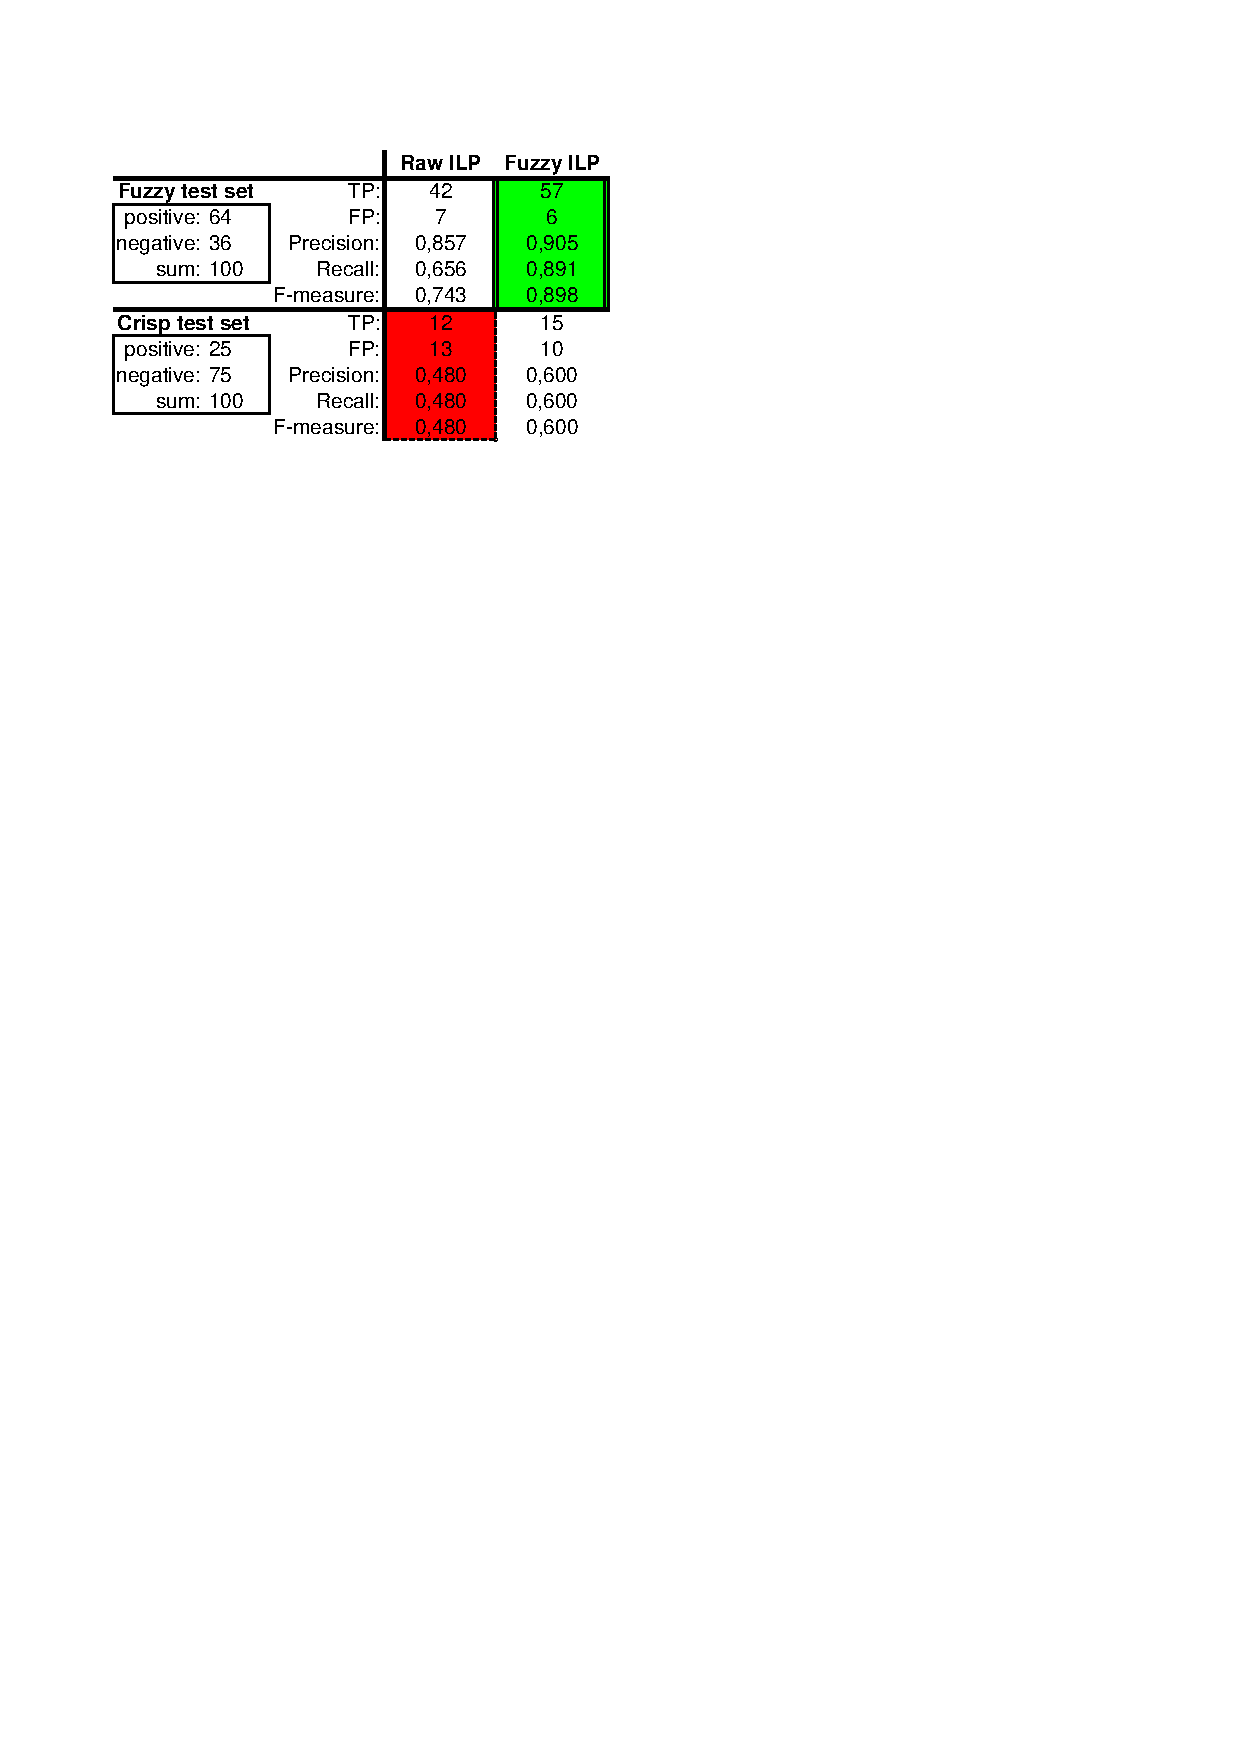
\includegraphics[width=0.75\hsize]{img/Evaluation}}
\bigskip
\begin{itemize}
	\item Rules evaluated on both testing sets.
		\begin{itemize}
			\item By use of conversion predicates (next slide)
		\end{itemize}
	\item Monotonized rules \alert{better in both cases}.
	\item Even better than \alert{other classifiers} (Znalosti 2010).
\end{itemize}
\end{frame}



\begin{frame}{Conversion of Results}
\setbeamercolor{block title}{bg=BrickRed}
\begin{block}{crisp $\rightarrow$ monotone}
\centerline{
\includegraphics[width=.8\hsize]{img/monot2nomon}}
\end{block}
\bigskip
\setbeamercolor{block title}{bg=OliveGreen}
\begin{block}{monotone $\rightarrow$ crisp}
\centerline{
\includegraphics[width=.8\hsize]{img/nomon2monot}}
\end{block}
\end{frame}

\section{Conclusion}
\begin{frame}{Summary}
 \begin{itemize}
  \item Proposed a system for extraction of semantic information 
  \item Based on linguistic tools for automatic text annotation
  \item Extraction rules adopted from \alert{Netgraph} application.
  \item ILP used for learning rules.
\bigskip
  \item Our future research will concentrate on:  
		\begin{itemize}
			\item \alert{Learning} of extraction rules.
			\item Extension of the method with WordNet technology.
			\item Adaptation of this method on \alert{other languages}.
			\item \alert{Evaluation} of the method.
		\end{itemize}
 \end{itemize}
\end{frame}

% no key words


\end{document}



%%% Local Variables: 
%%% mode: latex
%%% TeX-master: t
%%% End: 
